%!TEX root=../documentation-bachlorthesis-speicherarchitektur-lstucker.tex

\cleardoublepage
\chapter{Ist-Analyse}
Ziel der Ist-Analyse ist es, mit der Situationsanalyse den aktuellen Stand des bestehenden Systems bzw. der Speicherinfrastruktur zu beschreiben und zu bewerten.
Die Angaben für die Ist-Analyse wurden in diversen Interviews mit dem Auftraggeber und aus den von ihm gelieferten schriftlichen Dokumenten erhoben und zusammengestellt.

\section{Defintionen}

\subsection{Speichereinheit}
In der Arbeit werden die Angaben zu den Speichereinheiten anhand des SI-Standards \cite{Technology1998} verwendet, welcher zwischen Dezimal Präfixe, wie sie bei Festplatten angewendet werden, und Binär Präfixen unterscheidet.

\subsection{RAID 5}\label{RAID 5}

Ein RAID 5 Festplatten-Array besteht aus N identischen Festplatten auf welchen die Daten verteilt gespeichert sind. Die Einheit an Daten, welche auf derselben physischen Festplatte platziert ist, bevor weitere Daten auf eine andere Festplatte geschrieben werden, wird als eine Stripe-Einheit bezeichnet.
In der \refabb{abb:RAID 5 Architektur} wird eine Stripe-Einheit durch Blöcke dargestellt. Z.B. stellt A1 eine Stripe-Einheit dar. \cite{Kuratti1995}

Stripe-Einheiten, welche auf allen Festplatten verteilt denselben physikalischen Platz bzw. Adressbereich belegen, bezeichnet man als Stripe. In der \refabb{abb:RAID 5 Architektur} sind diese durch gleichfarbige Blöcke dargestellt. Hier repräsentieren z.B. die Stripe-Einheiten A1, A2, A3 und $A_{p}$ einen Stripe.
Jeder Stripe enthält mehrere Daten Stripe-Einheiten und eine Parität Stripe-Einheit. Eine Parität Stripe-Einheit ist eine XOR-Verknüpfung aller Daten Stripe-Einheiten eines Stripes. Durch die Speicherung und Berechnung einer Parität Stripe-Einheit pro Stripe, ermöglicht es in einem RAID 5 den Ausfall einer einzelnen Festplatte zu kompensieren. Die verlorenen Stripe-Einheiten der ausgefallenen Festplatte können durch das Lesen aller vorhandenen Daten Stripe-Einheiten und der Parität Stripe-Einheit der noch intakten Festplatten wiederberechnet bzw. rekonstruiert werden. Die Anzahl der Stripe-Einheiten eines Stripes ist durch die Stripe Width  ($W_{s}$) definiert. Die Anzahl der Daten Stripe-Einheiten in jedem Stripe ist durch $W_{s} -1$ definiert. \cite{Kuratti1995}

\begin{center}
\includegraphics[width=\linewidth, keepaspectratio = true]{media/Raid-5.png}
\mycaption{figure}{\label{abb:RAID 5 Architektur} RAID 5 Architektur \textit{RAID 5} \cite{Wikipedia2006}}
\end{center}

Die einzelnen Parität Stripe-Einheiten werden in rotierender Folge über die Festplatten verteilt. Dieses Verfahren trägt dazu bei, die I/O Last, welche durch Anfragen eine Aktualisierung der Parität veranlassen, auf die einzelnen Festplatten besser zu verteilen. Weil die Daten in einem RAID 5 auf mehrere Festplatten verteilt sind, erhöht sich die Wahrscheinlichkeit, dass eine Festplatte bei einer I/O Operation beteiligt ist, was wiederum den Datendurchsatz und die I/O Rate eines Array erhöht. \cite{Kuratti1995}

Für die Speicherung der Parität, muss ein Teil der gesamten Festplattenkapazität reserviert werden. Die für die Daten verfügbare Nettokapazität eines RAID 5 Arrays mit n Festplatten und s Speicherkapazität pro Festplatte lässt sich mit folgender Formel \cite{Kuratti1995} berechnen:

\begin{equation}
\mbox{Speicherkapaziät RAID 5}=(N-1)*S
\label{eqn:MTBF-RAID 5}
\end{equation}
 

\subsection{MTTR}
MTTR  ist die Abkürzung von "Mean Time To Recovery"' und bedeutet so viel wie die durchschnittliche Zeit, welche eine Komponente benötigt, um sich nach einem Fehler wieder herzustellen. Die MTTR in einen RAID 5 berechnet sich aus der Zeit bis eine Ersatzfestplatte installiert ist und der Disk Wiederherstellungszeit. 

\begin{equation}
MTTR_{RAID}=Replacement+Rebuild_{RAID}
\label{eqn:MTBF-RAID 5}
\end{equation}

Die Disk Wiederherstellungszeit in einem RAID 5 kann von den folgenden Faktoren abhängig sein:
\begin{itemize}
\item Anzahl der Festplatten
\item Speicherkapazität
\item Periodisierung der Rekonstruktion gegenüber dem normalen I/O
\item  normale I/O-Last während der Rekonstruktion
\item  CPU Last
\end{itemize}

Für die Ist-Analyse stehen keine aussagekräftigen Statistiken für die Disk Wiederherstellungszeit zur Verfügung. Es wird deshalb angenommen, dass heute eine allfällige MTTR 24 Stunden betragen würde.


\subsection{MTBF}
MTBF ist die Abkürzung von "Mean Time Between Failure"' und bedeutet so viel wie die durchschnittliche Betriebszeit einer Komponenten bis ein Fehler eintritt. Hersteller von Festplatten geben diesen Wert an, um die durchschnittliche Lebensdauer einer Festplatte zu beschreiben. 

Die MTBF mit n Festplatten berechnet man in einem RAID 5 \cite{Chen1994} wie folgt:
\begin{equation}
MTBF_{RAID 5}=\frac{MTBF_{Disk}^2}{N*(N-1)*MTTR_{Disk}}
\label{eqn:MTBF-RAID 5}
\end{equation}

\subsection{Verfügbarkeit}
Ein Service bzw. ein System gilt als verfügbar, wenn es seine dafür bestimmte Tätigkeit vollständig erfüllt. Die Wahrscheinlichkeit, in welcher ein Service in einer definierten Periode verfügbar ist, bezeichnet man als Verfügbarkeit \cite{Held2004}. Im Idealfall darf eine Service nie ausfallen und soll immer verfügbar sein. In der Realität ist eine perfekte Verfügbarkeit kaum gewährleistet. Es wird angestrebt, die erforderliche oder gewünschte Verfügbarkeit möglichst genau auszudrücken, damit mit Kennzahlen und Metriken die Verfügbarkeit definiert und gemessen werden kann. 

Die Verfügbarkeit wird aus dem Verhältnis der verfügbaren Zeit (Updatime) und der nicht verfügbaren Zeit (Downtime) eines Services \cite{Held2004} bemessen:

\begin{equation}
\mbox{Verfügbarkeit} = \frac{\mbox{Uptime}}{ \mbox{Downtime} + \mbox{Updatime} }
\label{eqn:Verfügbarkeit}
\end{equation}

\subsection{Datenverfügbarkeit}
Die Datenverfügbarkeit beschreibt die vom Hardware Speicherhersteller und dem Serviceanbieter als Speicherdienstleister "'Storage Service Provider (SSP)"'  gewährleistete Verfügbarkeit der Daten und die zugesicherte Antwortzeit beim Datenzugriff während dem Normalbetrieb \cite{TechTarget2001}.

In dieser Arbeit wird der Begriff dazu verwendet, die gewährleistete Verfügbarkeit für den Datenzugriff des Speichersystems zu beschreiben. Die Datenverfügbarkeit aus der Sicht des Endbenutzers der Webapplikation wird mit diesen Begriff nicht definiert. 

\subsection{Hochverfügbarkeit}
Die Autorin Andrea Held beschreibt in Ihren Buch den Begriff "Hochverfügbar" wie folgt:
\begin{quotation}\em
Ein System gilt als hochverfügbar, wenn eine Anwendung auch im Fehlerfall weiterhin verfügbar ist und ohne unmittelbaren menschlichen Eingriff weiter genutzt werden kann. In der Konsequenz heisst dies, dass der Anwender kein oder nur eine kurze Unterbrechung wahrnimmt.\end{quotation}\cite{Held2004}

Hardvard Research Group hat die Verfügbarkeit in Verfügbarkeitsklassen eingeteilt:

\begin{itemize}
\item Conventional (AEC-0): Funktion kann unterbrochen werden, Datenintegrität ist nicht essentiell
\item Highly Reliable (AEC-1): Funktion kann unterbrochen werden, Datenintegrität muss jedoch gewährleistet sein.
\item High Availability (AEC-2): Funktion darf nur innerhalb festgelegter Zeit beziehungsweise zur Hauptbetriebszeit minimal unterbrochen werden.
\item Fault Resilient (AEC-3): Funktion muss innerhalb festgelegter Zeiten beziehungsweise während der Hauptbetriebszeit ununterbrochen aufrechterhalten werden.
\item Fault Tolerant (AEC-4): Funktion muss ununterbrochen aufrechterhalten werden. Der 24*7 Betrieb (24 Stunden, 7 Tage die Woche) muss gewährleistet sein.
\item Disaster tolerant (AEC-5): Funktion muss unter allen Umständen verfügbar sein.
\end{itemize}
\cite{Held2004}

In der Arbeit werden zur Verfügbarkeitsbestimmung die Verfügbarkeitsklassen von Harvard Research Group verwendet.


\section{Bestandesaufnahme}
\subsection{Anwendungs-Architektur}
Die genaue Anwendungs-Architektur wird hier nicht beschrieben, da dies die Geschäftsgeheimnisse des Auftraggebers verletzen würde. Es werden deshalb nur die Teile davon beschrieben, welche die Geschäftsgeheimnisse des Auftragsgebers nicht verletzen.

Die Applikation ist eine Web-Applikation, welche auf dem Web-Framework Ruby On Rails aufsetzt.
Wie dem Namen "Ruby On Rails" zu entnehmen ist, basiert das Framework auf der Programmiersprache Ruby. Ruby ist eine dynamische, Objekt-orientierte, interpretierbare Programmiersprache, von Yukihiro Matsumoto 1995 hervorgebracht. Ein Ruby Programm benötigt für deren Ausführung keine Kompilation.

Ruby On Rails auch Rails oder RoR genannt, implementiert eine Model-View-Controller Architektur. Die drei Sub-Frameworks, spielen dabei eine signifikante Rolle in der Separierung des Codes: Active Record, Action View, und Action Controller. Die drei Sub-Frameworks sind auch im refabb{abb:Rails-Architektur} dargestellt (nach \cite{Bachle2007}).

\begin{center}
\includegraphics[width=\linewidth, keepaspectratio = true]{media/rails-architecure.png}
\mycaption{figure}{\label{abb:Rails-architektur}Rails Architektur \textit{RAID 5} \cite{Wikipedia2006}}
\end{center}

Beides, Ruby On Rails (auch nur "Rails" genannt) und Ruby sind Open-Source Programme. Die Quellprogramme sind für jeden Programmierer offen. Ruby wird unter der Lizenz "'Ruby License"' und GPL veröffentlicht, während Rails unter der "MIT License" veröffentlicht ist.

\subsection{System-Architektur}\label{System-Architektur}
Die bestehende System-Architektur besteht aus einem einzelnen Server, welcher von einem bekannten deutschen Webhosting-Provider gemietet wird. Beim gemieteten System handelt es sich um einen x64 Mikroarchitektur.

\subsection{Speicher-Architektur}
Die Speicher-Architektur besteht aus einem internen Block-basierendem RAID 5 Speicher. Die im Server verbauten Festplatten (RAID 5) werden mittels dem Linux Software RAID Kernel\footnote{\url{https://raid.wiki.kernel.org/}} und dem Verwaltungstool mdadm\footnote{\url{http://neil.brown.name/blog/mdadm}} zu einer logischen Einheit zusammengefasst. Für das RAID 5 werden drei  "'SATA 2"' Festplatten verwendet, welche jeweils eine Speicherkapazität von 2 Terabyte bzw. 1.818 Tebibyte aufweisen.

Im RAID Speicher ist ein root Dateisystem für das Betriebsystem, die Webapplikation, Datenbank, Logdateien und Bilddaten installiert.

\subsection{Speicherkapazität}
Die von RAID 5 zur Verfügung gestellte Speicherkapazität beträgt gemäss \refeqlb{eqn:RAID 5-3disk} 3.636 Tebibyte, davon sind nach Installation des Dateisystems $\approx 3.5$ Tebibyte bzw. $\ca. 3.8 $ Terabyte effektiv verfügbar. Davon sind anhand des \textit{df} Befehls,  wie im\reflisting{df} ersichtlich, $\ca. 2.5$ Terabyte für das Betriebsystem, die Webapplikation, Datenbank, Logdateien und Bilddaten reserviert. Als freier Speicherplatz verbleiben $\ca. 1.3$ Terabyte.

\begin{equation}
\mbox{Speicherkapazität RAID 5}= (3 - 1) * 1.818  \, \mathrm{TiB} =  3.636 \, \mathrm{TiB}
\label{eqn:RAID 5-3disk}
\end{equation}

\begin{lstlisting}[label=df, language=Bash, caption=Report Dateisystem Speicherplatz Belegung in Dezimal Prefix ]
root@www1:~# df -h
Filesystem            Size  Used Avail Use% Mounted on
simfs                      3.8T  2.5T  1.3T   67% /
\end{lstlisting}
\footnote{\url{http://www.debianadmin.com/manpages/dfmanpage.htm}}

\subsection{Datenwachstum}
Das \refabb{abb:disk-usage-by-year} zeigt den Speicherzuwachs von Mitte Juni bis Ende November.

\begin{center}
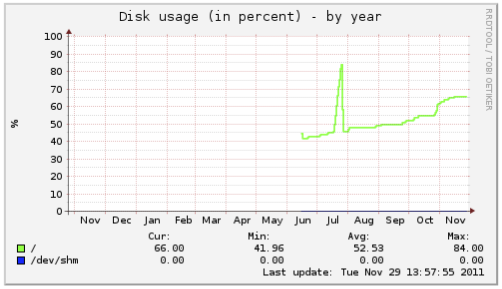
\includegraphics[width=\linewidth, keepaspectratio = true]{media/disk-usage-by-year.png}
\mycaption{figure}{\label{abb:disk-usage-by-year}Verhältnis von Speicheplatzverbrauch zur Speicherkapazität in Prozent in einer Zeitspanne von einen Jahr}
\end{center}

\subsection{Zugriffswachstum}
Für die Ist-Aufnahme konnten keine historischen Messdaten zur Verfügung gestellt werden.

\subsection{Skalierbarkeit Datenvolumen}
Während dem Betrieb ist ein Ausbau der Speicherkapazität (Skalierbarkeit) nicht möglich. Eine Vergrösserung der Speicherkapazität ist nur durch einen Wechsel auf ein anderes Hostingprodukt möglich. Dies erfordert eine Migration auf eine neue Server-Plattform. 

\subsection{Skalierbarkeit Datenzugriffe}
Keine Skalierbarung möglich. 

\subsection{Daten Durchsatz I/O}
Für die Ist-Aufnahme konnten keine Messdaten zur Verfügung gestellt werden.

\subsection{Daten Redundanz}

Die Daten-Redundanz wird durch das RAID 5 gewährleistet.

\subsection{Datenverfügbarkeit}
Stromausfälle und Netzwerkstörungen im Rechenzentrum des Hosting Providers führten zu Störungen und Ausfällen in der Webapplikation und in der Datenauslieferung. Die Störungen wurden jedoch nicht dokumentiert, weshalb keine statistische messbare Aussage über die erreichte Datenverfügbarkeit gemacht werden kann.

\subsection{Daten Sicherheit}
Die Daten sind durch physischen Fremdzugriff mittels Verschlüsselung geschützt. Für die Verschlüsselung wird das Device Mapper Module dm-crypt eingesetzt. dm-crypt verschlüsselt die Daten bereits auf Blockebene und ist somit für das Dateisystem transparent.

\subsection{Daten Integrität}
Zu jedem Bild wird eine Hash Checksumme gespeichert, die bei jedem Backup geprüft wird. Die Daten-Integrität ist somit sichergestellt.

\subsection{Backup}
Es wird täglich mittels dem Tool ccollect\footnote{\url{http://www.nico.schottelius.org/software/ccollect/}} ein R-Sync Backup der Daten erstellt. Das Backup wird ausser Hause gelagert.

\subsection{Wirtschaftlichkeit}
Die Kosten für die Speicherung der Daten inklusive Webinfrastruktur sind vergleichsweise zu alternativen Lösungen tief.

\subsection{Lokalität}

Die Web-Applikation inklusive dessen online Daten werden am selben Standort betrieben. Die Backupdaten werden an einen seperaten Standort gelagert. Der Zugriff auf Backup-Daten ist innerhalb 30 Minuten möglich.

\section{Analyse-Ergebnisse}

\subsection{System-Architektur}

\subsection{Datenwachstum und Speicherkapazität}
Die Messdaten aus dem  \refabb{abb:disk-usage-by-year} zeigen, dass das Datenvolumen seit  Juni 2011 bis Ende November 2011 mit Ausnahme einer unregelmässigen Spitze und einem grösseren Wachstumsschub Ende Oktober kontinuierlich zugenommen hat. Die etwas erhöhte Spitze lässt sich durch eine vorübergehende technische Änderung am System erklären und hat somit für die Auswertung keine Relevanz. Während der erwähnten Zeitspanne hat das Datenvolumen von 1,634 Terabyte auf 2,546 Terabyte zugenommen. Dies entspricht einer Datenzuwachsrate von 0,912 Terabyte bzw. 55,8\% in fünf Monate. Das Durchschnittliche Datenwachstum beträgt 0,182 Terabyte bzw. 11,1\% pro Monat.

Setzt sich der bisherige Trend fort, so ist die verfügbare Speicherkapazität von 3,8 Terabyte in weniger als 7 Monate erschöpft. Berücksichtigt man bei diesem durchschnittlichen Datenwachstum mögliche Wachstumsschübe für Neukunden, welche durch das Einlesen von deren bestehende Bilddatenbanken entstehen könnten, so reduziert sich die Kapazitätsreserve nach unten und würde eine vorzeitige Umstellung auf ein neues System bedingen.

Gemäss des Auftraggebers ist ferner ein neues Feature für die Web-Applikation geplant, welches den Speicherplatzbedarf verdoppeln würde. Die aktuelle Speichersituation lässt momentan den produktiven Einsatz des neuen Feature nicht zu. Das durchschnittliche Datenwachstum würde voraussichtlich auf 0,364 Terabyte pro Monat steigen.

Die jetzige Speicherkapazität erfüllt schon heute die Anforderungen nicht mehr.

\begin{equation}
\mbox{Datenwachstum}_{Monate5} = 2,546  \mathrm{TB} - 1,634 \mathrm{TB} =  0,912 \mathrm{TB}
\label{eqn:Verfügbarkeit_5Monate}
\end{equation}

\begin{equation}
\mbox{Datenwachstum}_{Monate5} = \frac{0,912 \mathrm{TB}}{\frac{1,634 \mathrm{TB}}{100 \%}} =  55,813\%
\label{eqn:Verfügbarkeit_5Monate_in_Prozent}
\end{equation}

\begin{equation}
\mbox{Durchschnittliches Datenwachstum}_{Monate} = \frac{0,912 \mathrm{TB}}{5\mathrm{m}} =  0,1824 \mathrm{TB}
\label{eqn:Verfügbarkeit_1Monate}
\end{equation}

\begin{equation}
\mbox{Durchschnittliches Datenwachstum}_{Monate} = \frac{55,813\%}{5 \mathrm{m}} = 11,162\%
\label{eqn:Verfügbarkeit_1Monate_in_Prozent}
\end{equation}

\subsubsection{old}
Betrachtet man die erwähnte Zeitspanne hat das Datenvolumen in Bezug zur Speicherkapazität von 40\% (1556 Gibibyte bzw. 1.5 Tebibyte) auf beinahe 67\% (2568 Gibibyte bzw. 2.5 Tebibyte) in 5 Monaten zugenommen. Das durchschnittliche Datenwachstum beträgt somit gemäss Messdaten pro Monat ca. 5\% (195 Gibibyte bzw. 0.19 Tebibyte). Geht man davon aus, das sich das Datenwachstum auf dem gleichen Niveau vorsetzt, ist die Speicherkapazität innert 5 Monate ausgeschöpft.

Ein geplantes neues Feature der Web-Applikation würde den Speicherplatzbedarf verdoppeln. Aufgrund der Vorhanden Speicherkapazität kann das Entwickelte Feature zur Zeit nicht Produktive verwendet werden. Nach Inbetriebnahme des Feature würde sich das Datenwachstum um den Faktor 2 auf 390 Gibibyte steigern.

\subsection{Skalierbarkeit Datenvolumen}\label{AnalyseSkalierbarkeitDatenvolumen}
Die Eingesetzte Speicherarchitektur lässt eine Skalierung des Datenvolumen mittels hinzufügen von weiteren Festplatten oder durch Migration auf grösseren Festplatten zu. Die maximale Anzahl von Festplatten wird dabei durch die Anzahl vorhandenen SATA Anschlüsse im Server bestimmt. Beim eingesetzten Server handelt sich um eine Hosting Produkt welche meist begrenzt ausbaubar ist. Bei Hosting Produkte erfolgt eine Skalierung meist durch eine Wechsel auf eine besser ausgebautes Hosting Produkt. 

\subsection{Skalierbarkeit Datenzugriffe}
Eine mögliche Skalierung bezüglich des Datendurchsatzes könnte durch schnellere Festplatten, durch eine optimierte Verteilung der I/O-Operationen auf verschiedene Festplatten oder durch die Verteilung der Daten auf weitere Systeme erreicht werden. Zu beachten sind auch hier dieselben Prämissen, wonach wie beim Ausbau des Datenvolumens das bestehende System nur sehr begrenzt ausgebaut werden kann bzw. auf ein anderes Hostingprodukt migriert werden müsste.

\textbf{Skalierung durch schnellere Festplatten:}
Moderne Festplatten, mit Ausnahme von den teuren Solid State Disk (SSD), bieten zwar eine grössere Speicherdichte aber aufgrund der erreichten physikalischen Grenzen keine bedeutend effizientere IOPS versprechen. Eine Festplatte mit 7200 RPM erreicht durchschnittlich ein IOPS zwischen 75 und 100 IOPS. Bei SSD Disks wurden schon 1'190'000 IOPS in einem einzelnen PCI Geräte gemessen.\cite{Symantec2011} \cite{Fusionio} 
Ein Wechsel auf die genannten SSD Festplatten, ist aktuell noch mit sehr hohen Kosten pro Gigabyte verbunden. Gartner geht davon aus, dass 2012 die Preise pro Gigabyte bei SSD auf durchschnittliche 1\$ sinken werden. Gegenüber den heutigen Preisen bei konventionellen Festplatten von 30 Cents pro Gigabyte ist dies immerhin 3x teurer. Aus diesem Grund werden SSD Disks bei grossen Datenvolumen meist noch nicht eingesetzt, ausser spezielle Anforderungen an die Performance rechtfertigen die höhere Investition. \cite{AgamShah2011}

\textbf{Skalierung duch Verteilung der I/O Operationen:}
Ein RAID oder Volume Manager bietet die Möglichkeit, die I/O Operationen auf mehrere Festplatten zu verteilen. In einem RAID 5 verkleinert sich wie in Kapitel \refchap{AnalyseSkalierbarkeitDatenvolumen} beschrieben, die MTTF mit jeder weiteren Festplatte. Zudem sind die verfügbaren Anschlüsse in einem Server ebenfall ein zu berücksichtigen limitierender Faktor.

\textbf{Skalierung durch Verteilung der Daten:}
Nicht alle Kategorien von Daten haben die gleichen Anforderungen an den Durchsatz. Datenbanken z.B. benötigen in der Regeln einen höheren IOPS als statische Daten wie z.B. Bild-Daten, welche weniger oft abgefragt werden. Für die Verteilung der Daten ist eine Änderung in der System-Architektur und allenfalls in der Anwendungs-Architektur notwendig. Ein Beispiel für eine solche Anpassung der System-Architektur wäre die Auslagerung der Datenbank auf ein separates System, welches mit schnellen Solid State Disk ausgerüstet ist. 

\subsection{Redundanz}
Eine RAID 5 System bietet wie im \refsec{RAID 5} beschrieben, keine 1:1 Redundanz. Die Daten sind im RAID 5 nicht doppelt gespeichert, sondern werden bei einen Datenverlust mittels XOR Operation aus den Parität Stripes und den vorhandenen Daten Stripe-Einheiten berechnet. 

Bei einen Zugriff auf einen verlorenen Daten Stripe werden die Daten online berechnet. 

Treten bei einer Festplatte Fehler auf, werden die verlorenen Daten bei einem Zugriff aus dem Parität Stripe Einheit.??? Der Zugriff auf die Daten ist durch die Berechnung der Daten aus dem Parität Stripe Einheit Online möglich. Wird die ausgefallen Festplatte durch eine neu intakte Festplatte ersetzt, können die Daten durch einen Rebuild während des Betriebs wieder hergestellt werden. Durch die Berechnung und Schreib/Lese Operationen im RAID während des Wiederherstellungprozesses verschlechtert sich der Datendurchsatz und I/O Rate für den Datenzugriff wesentlich.

Einen Ausfall einer weiteren Festplatten kann das RAID 5 System nicht mehr kompensieren und führt zu einem physischen Datenverlust aller Online-Daten. Die Daten müssen in der Folge mittels des Backups eingelesen und wiederhergestellt werden, was jedoch nur im Offline-Betrieb möglich ist. 

Bei Festplatten welchen aus dem gleichen Produktionszyklus stammen, kann die Wahrscheinlichkeit eines weiteren Ausfall höher sein, im vergleich zu Festplatten die aus unterschiedlichen Produktionszyklen stammen.

\subsection{Service- und Daten-Verfügbarkeit}
Die bisherige System-Architektur gemäss dem Ist-Bestand ermöglichen keine AEC-2 Hochverfügbarkeit. Grund dafür ist die Fokussierung auf einen einzelnen Server in der System-Architektur. Der Server stellt eine "'Single Point of Failure"' (SPOF) dar. Tritt beim Server eine Störung auf, wie Sie zum Beispiel Aufgrund eines Gerätedefekts oder Softwarefehler auftreten können, kann der Service nicht von einem redundantem System übernommen oder weitergeführt werden. Eine Störung kann also die Verfügbarkeit während den Betriebszeiten starl gefährden und entspricht nicht den heutigen Anforderungen.

Die Netzwerkverfügbarkeit wird vom Hosting Anbieter gemäss den Allgemeinen Geschäftsbedingungen \cite{Ag2009} mit einer Verfügbarkeit von 99\% im Jahresmittel gewährleistet. Die Verfügbarkeit könnte somit bei einem 24x365 Stunden Betrieb während 87,6 Stunden nicht gewährleistet sein.

Das Speichersystem für sich selbst betrachtet kann die Verfügbarkeit und die Daten-Integrität gewährleisten, sofern keine Störungen durch einen Festplattendefekt eintreten. Das Speichersystem, welches ein interner Block-basierenden RAID 5 Speicher darstellt, ist ein Bestandteil des Serversystems und weist deshalb die selbe Verfügbarkeitsstufe wie das Serversystem auf. Die Service und Datenverfügbarkeit weist aus den genannten Gründen eine Verfügbarkeit Stufe von '"Highly Reliable"' AEC-2 auf.
\subsubsection{old}

Die Verfügbarkeit der restlichen Infrastrukturkomponenten und Systeme sind in diesem Bericht nicht aufgenommen worden (out of scope).
 \cite{Ag2009} Der Auftraggeber muss für diese Komponenten selber für die geforderte Verfügbarkeit besorgt sein.

Die im \refsec{System-Architektur}  beschriebene System-Architektur gewährleistet keine Hochverfügbarkeit der Daten. Einer der Gründe dafür ist, dass die Applikation nur auf einem einzelnen Server betrieben wird, dessen Hardware mit Ausnahme der Festplatten keine Redundanz aufweist und nicht für Hochverfügbar ausgelegt ist. 

Die Applikation wird auf einem einzelnen Server betrieben. Der Server und dessen Hardware mit Ausnahme der Festplatten stellen einen "'Single Point of Failure"' (SPOF) dar. Fällt der Server wegen eines Hardwaredefektes oder einem Softwarefehler aus, sind Daten und Anwendung für den Endbenutzer nicht mehr verfügbar.

Zudem werden die Daten und Applikation nur an einem Standort betrieben. Treten unvorhersehbare Ereignisse auf, wie z.B. ein lokaler Stromausfall, ein Brand oder eine Naturkatastrophe, kann der Betrieb nicht ohne die Wiederherstellung des ganzen Systems inklusive Daten von Backup wieder aufgenommen werden. Sofern nicht ein gemieteter Ersatzserver bereitsteht, muss ebenfalls die Beschaffung und Installation eines neuen Systems bei einem anderen Hosting Provider zur Ausfallzeit (Downtime) mit einberechnet werden. Der Service wäre während einer längeren Zeit nicht mehr verfügbar. Ein Kundenverlust und weitere Konsequenzen könnten die Folge sein.

\subsection{Daten Sicherheit}
Durch die Festplattenverschlüsselung sind die Daten bei abgeschaltetem Server vor unberechtigten Zugriffen geschützt. Befindet sich der Server jedoch im laufenden Betrieb, bietet die Verschlüsselung keinen Schutz vor Datendiebstahl. 

In einem Interview mit Ben Schwan im Technology Review hat Edward W. Felden, Professor für Informatik an der Princeton University den Grund dafür erklärt. 

\begin{quotation}\em
... ,die Dechiffrierungsschlüssel bei einer Festplattenverschlüsselung sitzen immer irgendwo im DRAM-Speicher. Um an sie heranzukommen, schaltet der Angreifer zunächst den Strom des Rechners aus und stellt die Energieversorgung dann gleich wieder her. Dann bootet er die Maschine in ein spezielles, böswilliges Betriebssystem hinein. Zu diesem Zeitpunkt enthält der Speicher noch immer die Originalinformationen, die verfügbar waren, als der Rechner noch nicht abgeschaltet wurde – die gewünschten Schlüssel natürlich auch. Das kurze Abschalten des Stroms hat daran rein gar nichts geändert. Der Angreifer kann dann die gewünschten Dechiffrierungsschlüssel aus dem Speicher auslesen und damit die geschützten Informationen auf der Festplatte jederzeit entschlüsseln\end{quotation}\cite{Schwan2008}

Des weiteren bietet eine Festplatten keinen Schutz bei Schwachstellen in der Software oder  der Konfiguration im laufenden Betrieb. Grund dafür ist, dass das Betriebsystem und Anwendungen über eine Verschlüsselungsschicht unverschlüsselt zugreifbar sind.

\subsubsection{old}
--- Skalierbarkeit Datenvolumen ---
Bei Hosting Angeboten bezieht man in Normalfall fertige Produkte, die sich im Server-Typ, Grösse des Speichers, der Anzahl Festplatten, CPU und Memory unterscheiden. Benötigt man für seine Applikation mehr Leistung oder einen grösseren Speicher muss man das Produkt wechseln, was meist mit einer Migration auf einen anderen Server verbunden ist.

Die jetzige Speicher- und Applikations-Architektur ist auf dem Betrieb auf einem einzelnen Server ausgelegt. Für die Skalierbarkeit des Datenvolumen bedeutet diese, dass man das Datenvolumen nur durch grössere Festplatten oder durch eine grössere Anzahl von Festplatten ausbauen kann. 

